\subsection{Grayscale to RGB}
\begin{figure}[!hbt]
    \centering
    \begin{minipage}{0.45\textwidth}
        \centering
        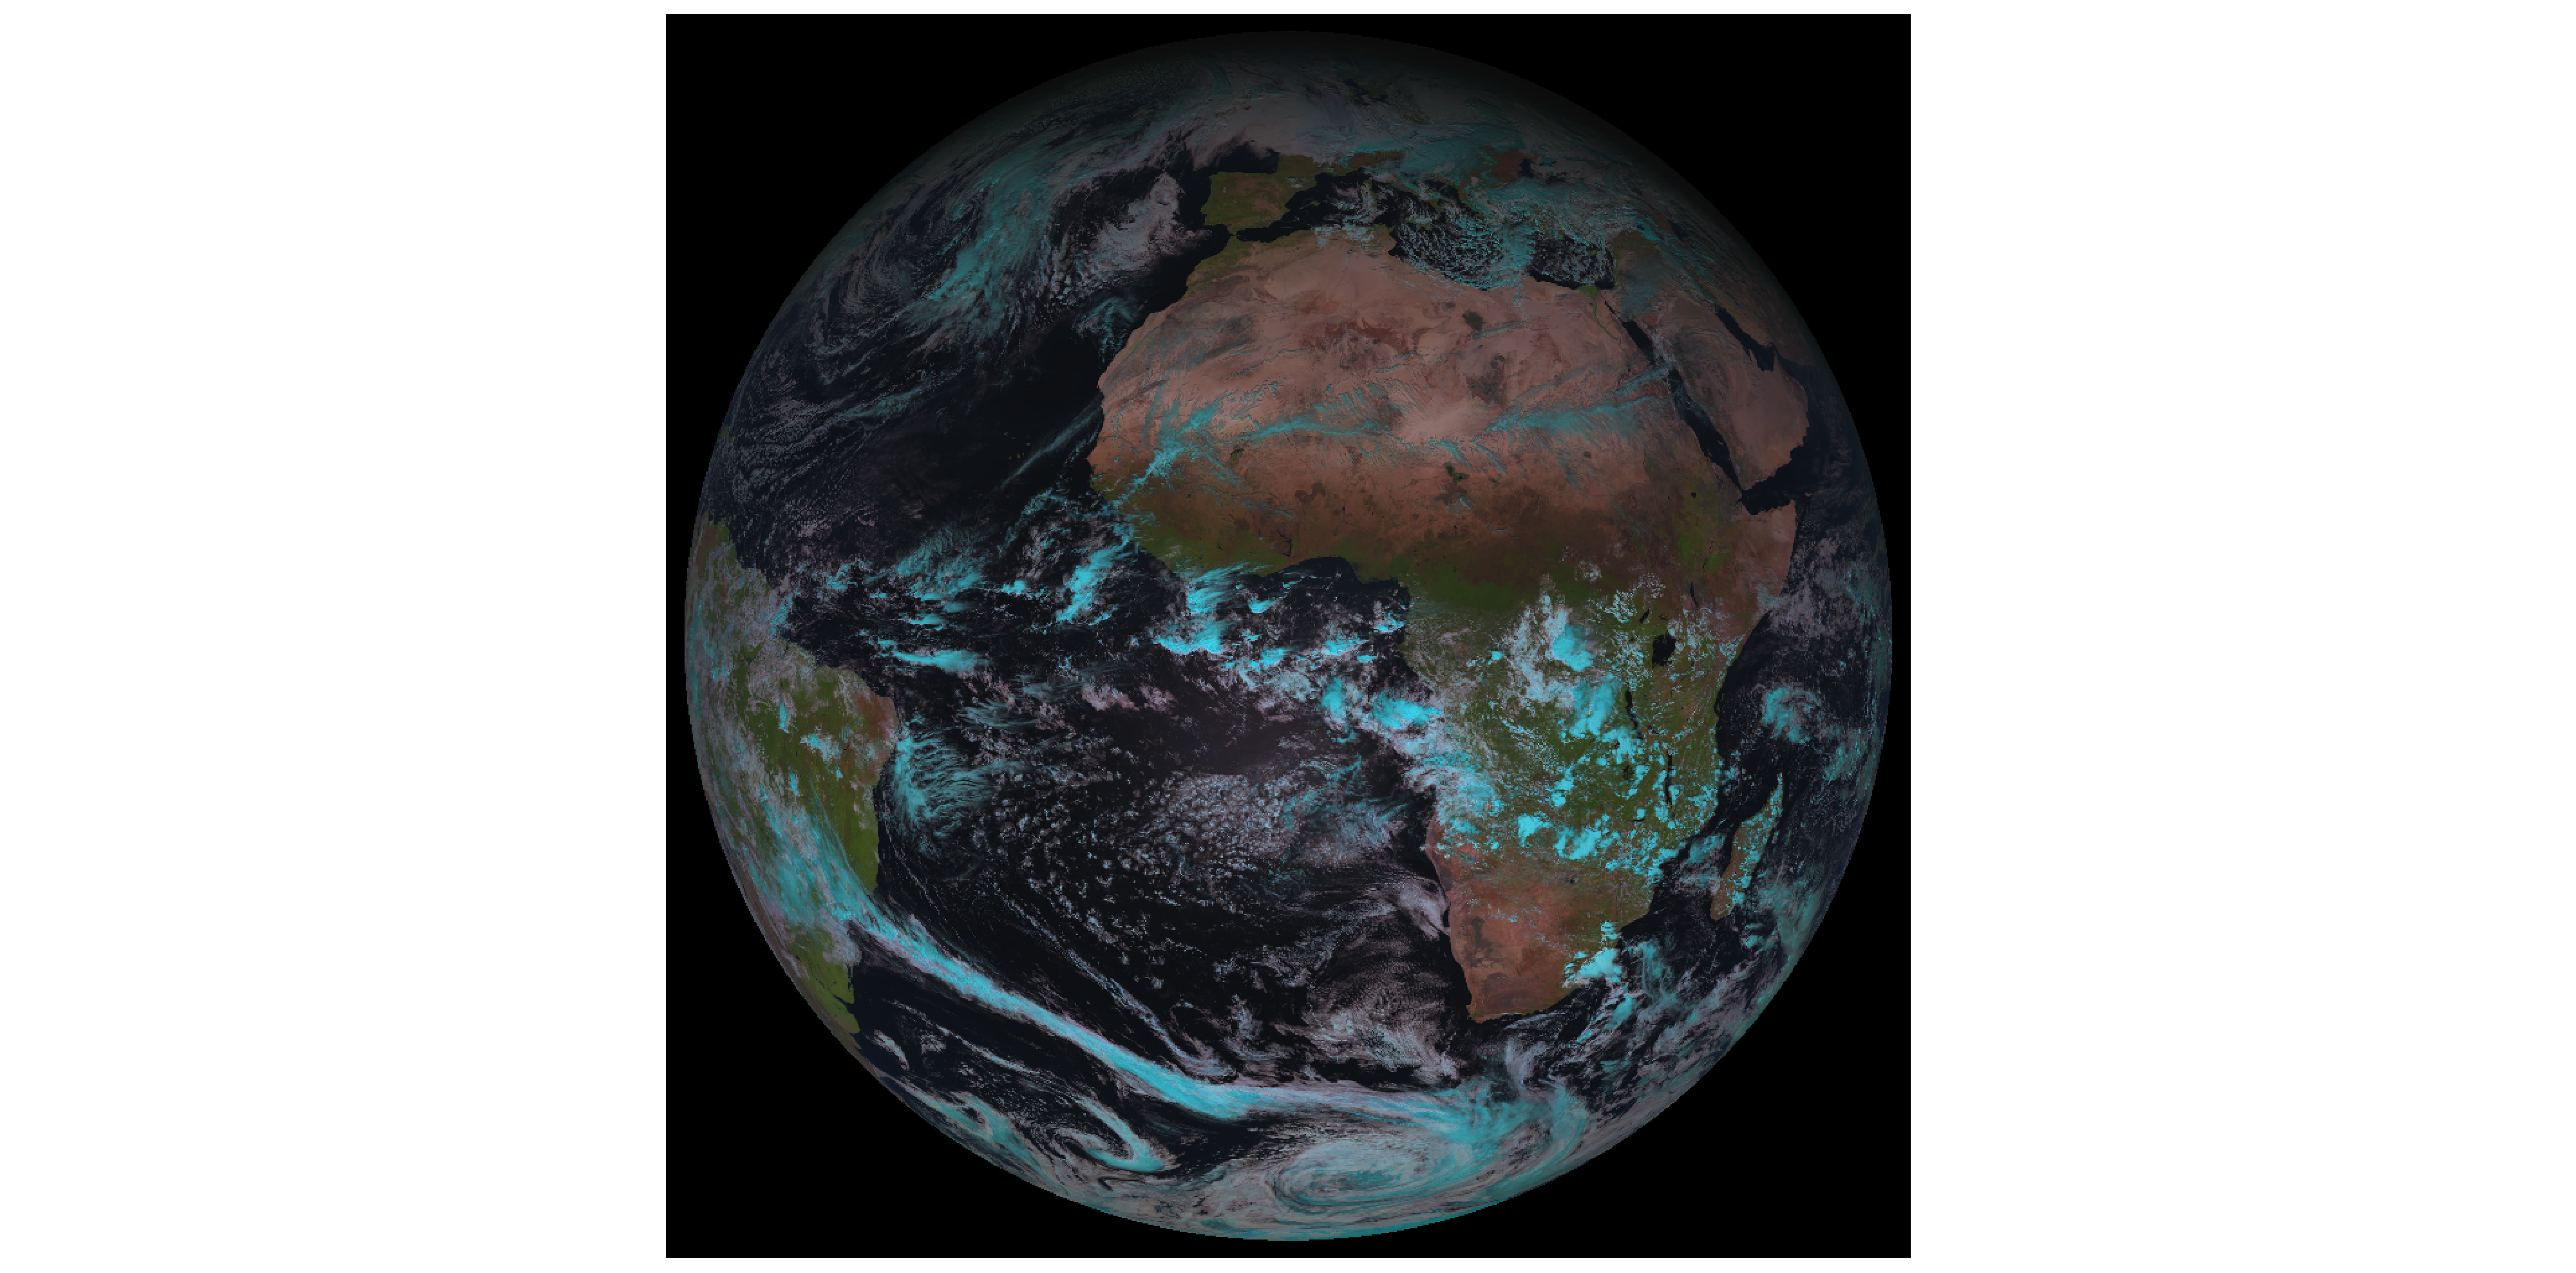
\includegraphics[width=0.9\textwidth]{2019-01-05 122743.pdf}
        \caption{RGB created from the stacking of the IR 1.6, VIS 0.6 and VIS 0.8 channel images for 2019-01-05 12:27:43 }
        \label{fig:av_rgb}
    \end{minipage}\hfill
        \begin{minipage}{0.45\textwidth}
        \centering
        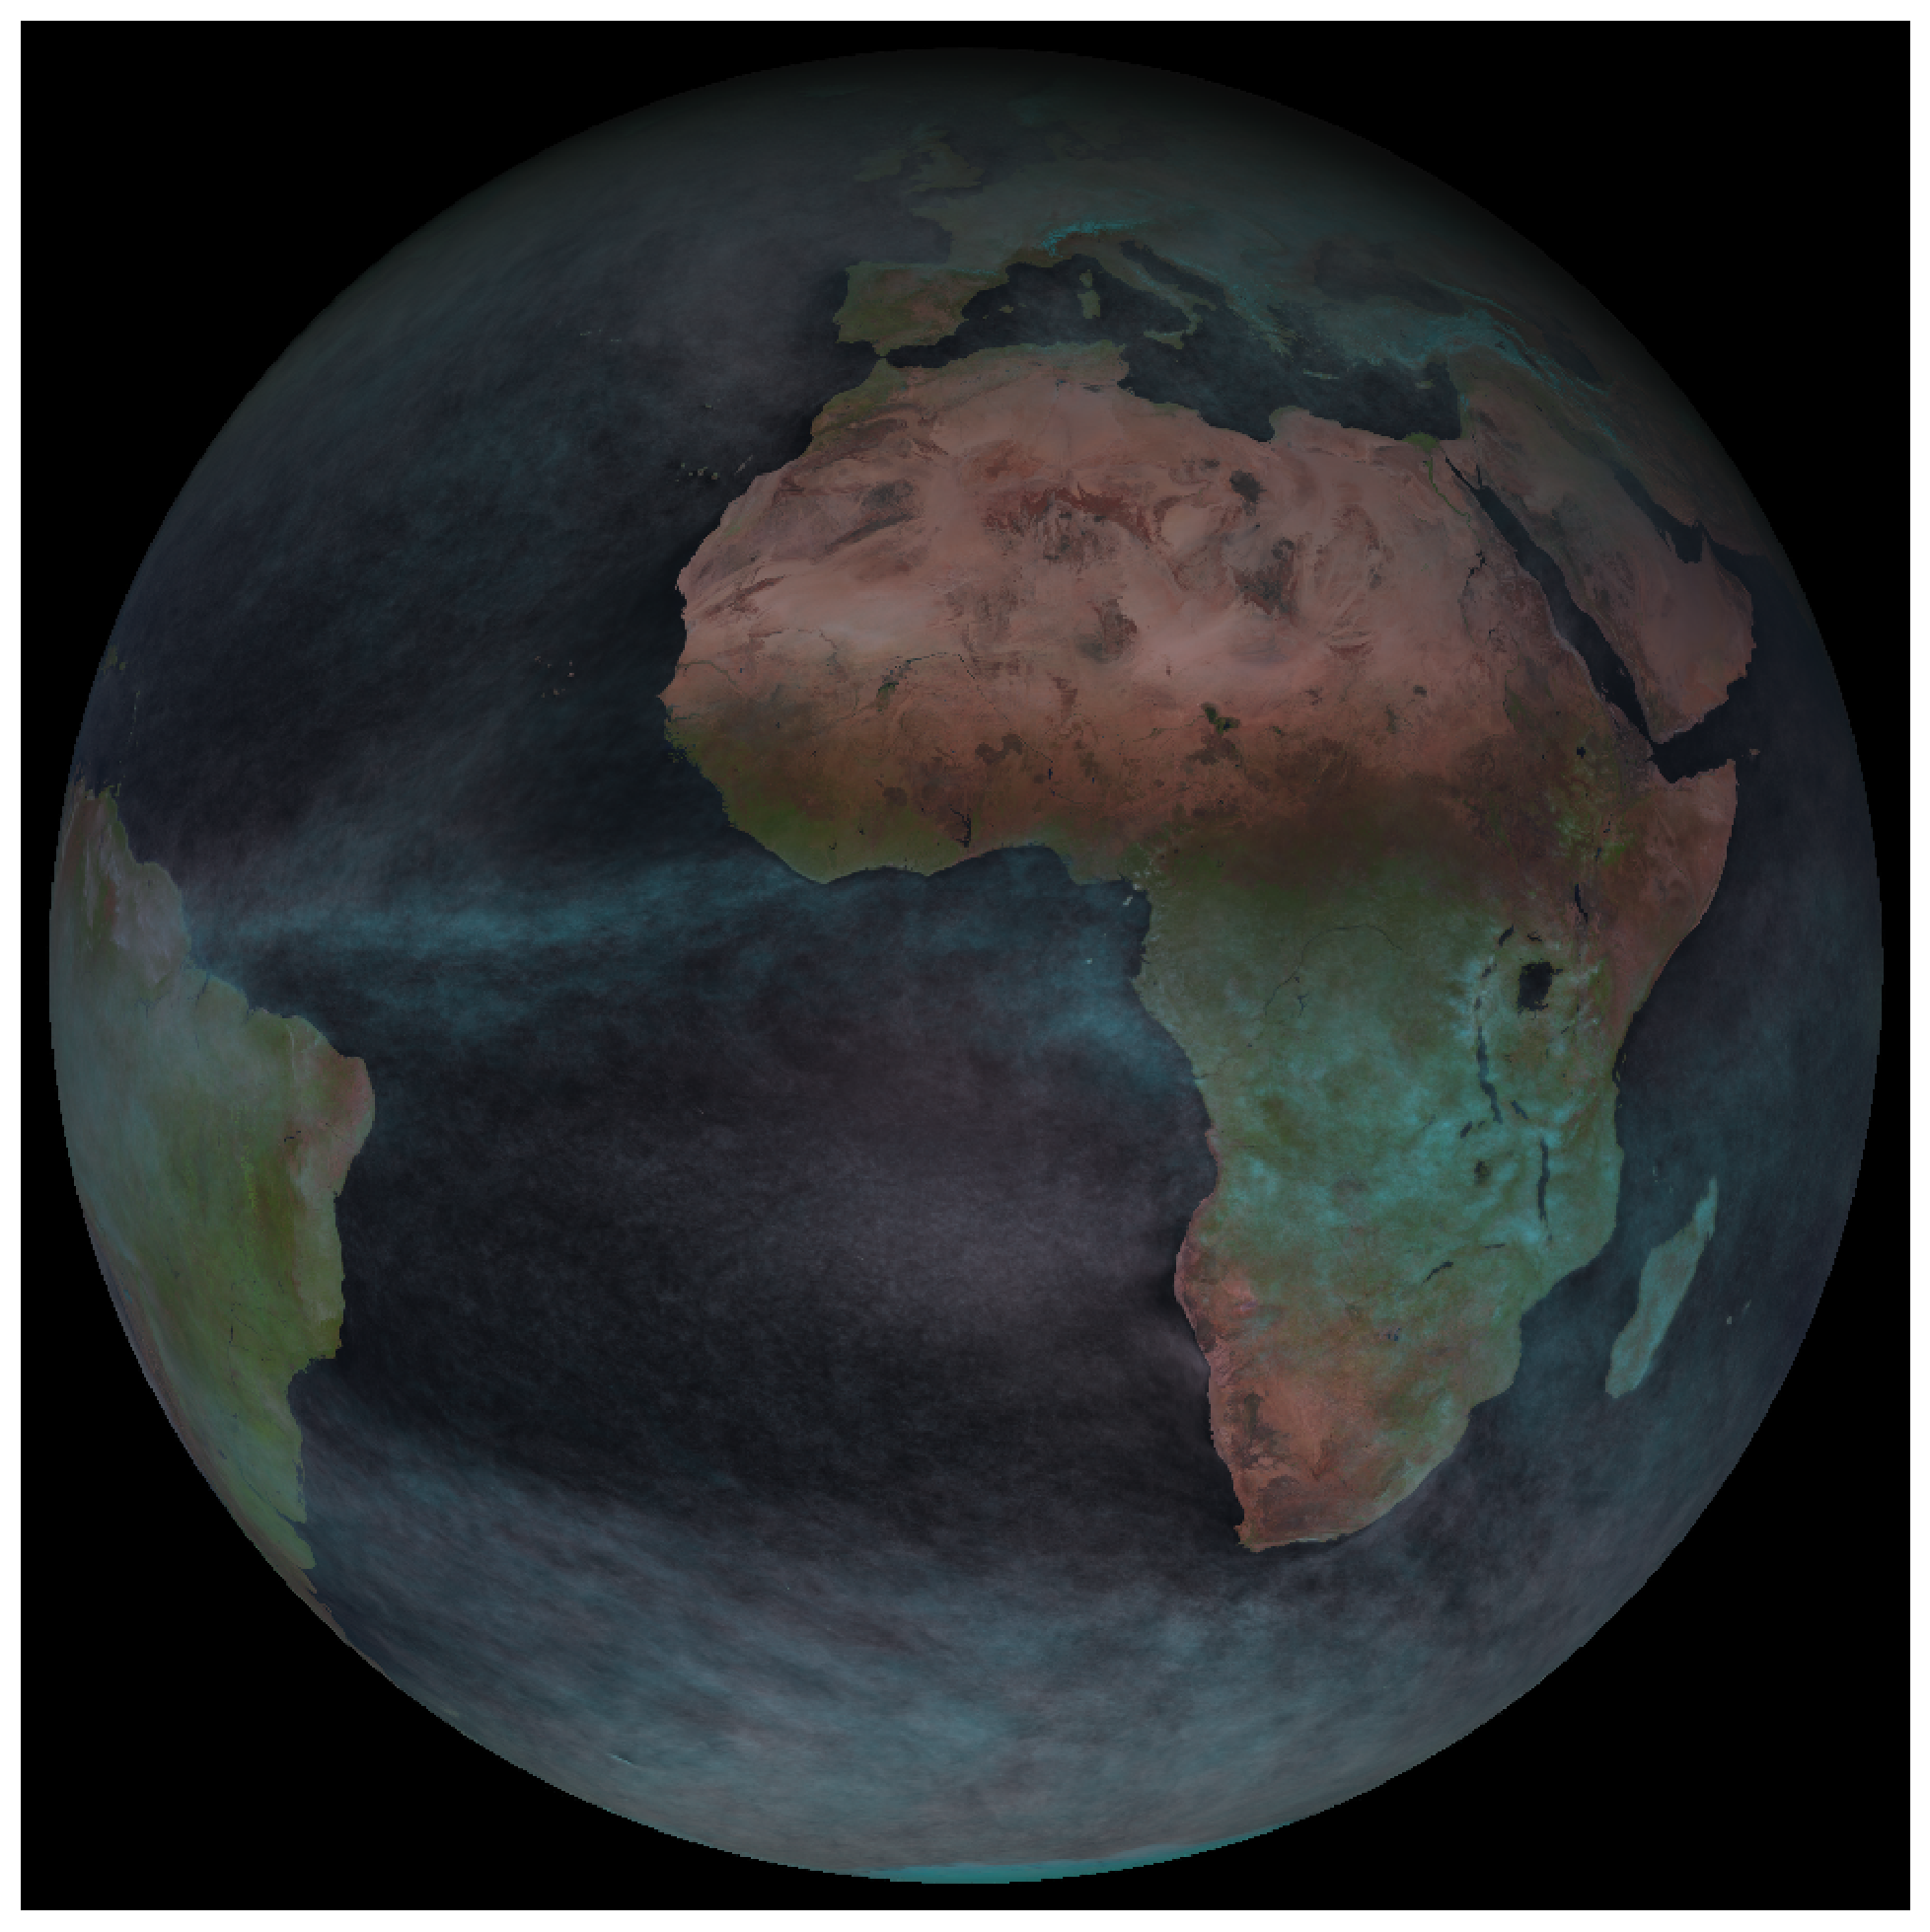
\includegraphics[width=0.9\textwidth]{2019-01-05 122743_av.pdf}
        \caption{RGB image formed from the averaging of all pixel values across the month of January 2019}
        \label{fig:av_cloud}
    \end{minipage}\hfill
\end{figure}

Fig.~\ref{fig:av_rgb} and Fig.~\ref{fig:av_cloud} both show an RGB colour image of the Earth in January 2019, created from data taken from Meteosat 9. The former consists of an RGB image, plotted using the channel data obtained at 12:27:43 on the 5th Janury 2019, while the latter was created through the addition and subsequent division of the corresponding pixel values across all the images taken in the month of January 2019. 


\subsection{Cloud Removal Using Thresholding}
\begin{figure}[hbt!]
    \centering
    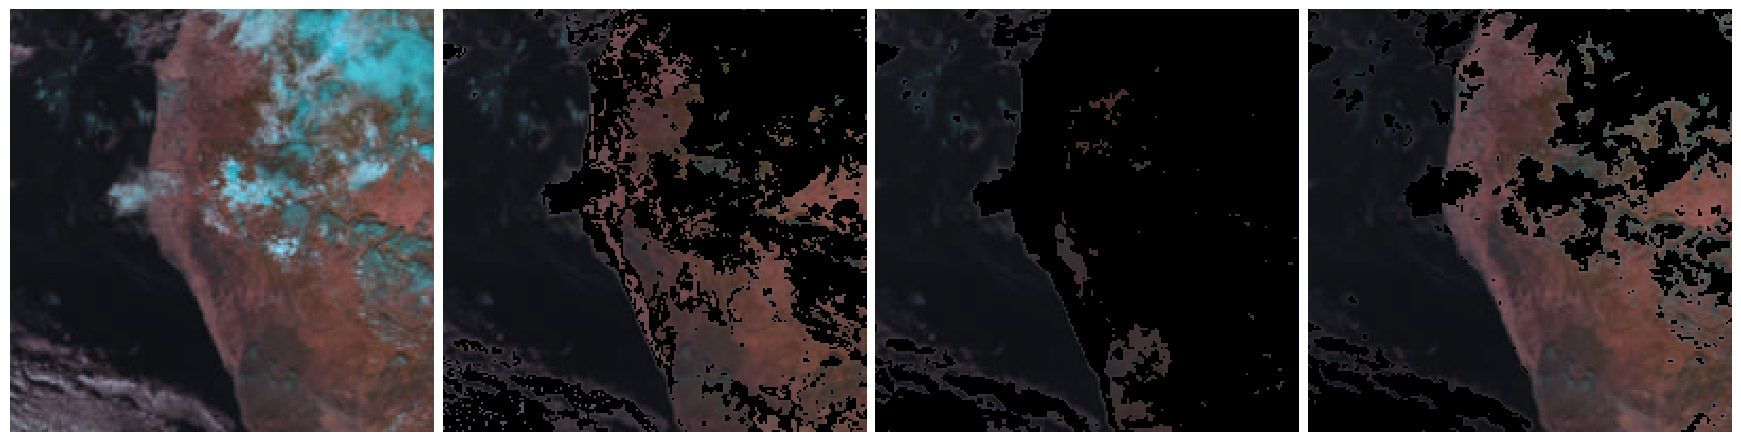
\includegraphics[width=1\textwidth]{compare_removal.png}
    \caption{Comparison of cloud removal algorithms on image from 2019-01-05 12:27:43.
    \\From left to right: original RGB image, thresholded image with values determined via inspection, thresholded image with single Otsu threshold value, and thresholded image using Otsu threshold values determined via use of masks over sea and land}
    \label{fig:iterav}
\end{figure}


Fig.~\ref{fig:iterav} illustrates the implementation of the different cloud removal methods we used to reduce pixel cloud noise, and shows their relative effectiveness. The three images on the far right of the figure are all RGB images in which a different thresholded mask was applied to each one. From left to right the masks were calcualted using threshold values determined by inspection, Otsu's algorithm, and the combination of Otsu's algorithm and a landmask. The separability measure of the global Otsu algorithm, the image second from the right, was calculated using Eq.~\ref{eq:sepm} and found to be $\eta = 0.932$.

\begin{figure}[hbt!]
    \centering
    \includegraphics[width=1\textwidth]{g_Otsu_sealand_fail.png}
    \caption{Implementation of Otsu's algorithm. From left to right: Original greyscale image calculated from the square root of the mean sum squared of each channel (IR 1.6, VIS0.6, and VIS 0.8), histogram of distribution of pixel intensity values with red vertical line indicating the Otsu threshold value calculated, and thresholded mask determined from Otsu's algorithm}
    \label{fig:g_Otsu_fail}
\end{figure}

\begin{figure}[hbt!]
    \centering
    \includegraphics[width=1\textwidth]{landmask_Otsu_threshold_2019-01-05 122743.png}
    \caption{Implementation of Otsu's algorithm over the land using a landmask. From left to right: Original greyscale image of VIS 0.6 channel, histogram of distribution of pixel intensity values with red vertical line indicating the Otsu threshold value calculated, and thresholded mask over land determined from Otsu's algorithm}
    \label{fig:bOtsu_land}
\end{figure}

\begin{figure}[hbt!]
    \centering
    \includegraphics[width=1\textwidth]{seamask_Otsu_threshold_2019-01-05 122743.png}
    \caption{Implementation of Otsu's algorithm over the sea using a reversed landmask. From left to right: Original greyscale image of VIS 0.8 channel, histogram of distribution of pixel intensity values with red vertical line indicating the Otsu threshold value calculated, and thresholded mask over sea determined from Otsu's algorithm}
    \label{fig:bOtsu_sea}
\end{figure}

Fig.~\ref{fig:g_Otsu_fail}, Fig.~\ref{fig:bOtsu_land} and Fig.~\ref{fig:bOtsu_sea} each show three plots that demonstrate the process of Otsu's threshold determination. From left to right we have the original greyscale image upon which Otsu's algorithm is performed, a histogram of the frequency of occurrence of different pixel values with a red vertical line indicating the calculated optimum threshold value, and the final thresholded mask determined from this value. Fig.~\ref{fig:g_Otsu_fail} shows the calculation of one threshold value for a set datetime, whilst Fig.~\ref{fig:bOtsu_land} and Fig.~\ref{fig:bOtsu_sea} show the workings of the algorithm over the land and sea masked images respectively.\\

\begin{figure}[hbt!]
    \centering
    \includegraphics[width=0.5\textwidth]{Otsu_av_mon.png}
    \caption{Averaged RGB image for January 2019 after the removal of cloud cover using land masks and Otsu's algorithm for optimum threshold identification}
    \label{fig:av_Otsu}
\end{figure}


Fig.~\ref{fig:av_Otsu} shows the cloud free averaged image for the month of January 2019 via use of our masked Otsu's algorithm (steps shown above in Fig.~\ref{fig:bOtsu_land} and Fig.~\ref{fig:bOtsu_sea}) revealing a clearer view of the terrain on the Earth's surface below the cloud cover. Some missing pixels can be observed towards the top of the coastline.\\

\begin{figure}[h]
    \centering
    \includegraphics[width=0.5\textwidth]{Otsu_filled_2019-01-05 122743.png}
    \caption{New cloud free image for 2019-01-05 12:27:43, where cloudy pixels have been replaced by the corresponding pixels in the averaged January cloud free image}
    \label{fig:Otsu_fill}
\end{figure}

Using Fig.~\ref{fig:av_Otsu}, Fig.~\ref{fig:Otsu_fill} shows an example of a thresholded image where the cloud cover pixels have been replaced by their average cloud-free pixel value for the month of January. The image looks noisier than the previously averaged image due to the presence of some areas of cloud cover that were not selected by the calculated threshold value.\\

\subsection{Percentage Cloud Cover Change}

Fig.~\ref{fig:cloud_pc_jan} shows a plot of the change in percentage cloud cover over the course of the month of January 2019 for an area in the Southern Hemisphere above the Atlantic Ocean. The plot shows consistently high values of cloud cover with an average value of approximately 40 percent. The percentage cloud cover values plotted here were calculated using masks generated from the inspection thresholding method. Two images taken 15 minutes apart were plotted per day (except for the 29th January 2019) providing us with a visual representation of a measure of the error range on the plot.
\begin{figure}[hbt!]
    \centering
    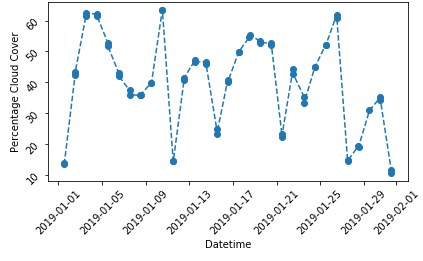
\includegraphics[totalheight=0.3\textheight]{cloud_percent_jan_southsea_not.png}
    \caption{Plot of the change in cloud cover percentage over the course of January 2019 for an area over the Atlantic Ocean in the Southern Hemisphere}
    \label{fig:cloud_pc_jan}
\end{figure}

\begin{figure}[!hbt]
    \begin{minipage}{0.48\textwidth}
        \centering
        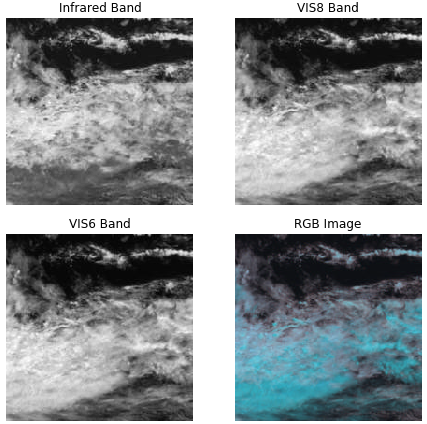
\includegraphics[width=1\textwidth]{60_per_day_sea_not.png}
        \caption{Images of the three channels (IR 1.6, VIS 0.8, VIS 0.6) and the calculated RGB image for 2019-01-10 12:27:43, corresponding to the data point indicating $~$60 percent cloud cover in Fig.~\ref{fig:cloud_pc_jan}}
        \label{fig:60pc}
    \end{minipage}\hfill
    \begin{minipage}{0.48\textwidth}
        \centering
        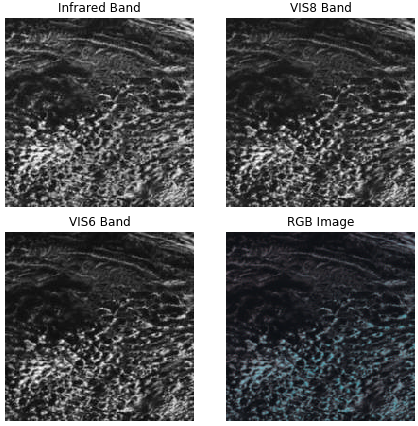
\includegraphics[width=1\textwidth]{15_per_day_sea_outlier_not.png}
        \caption{Images of the three channels (IR 1.6, VIS 0.8, VIS 0.6) and the calculated RGB image for 2019-01-11 12:27:43, corresponding to the data point indicating $~$15 percent cloud cover in Fig.~\ref{fig:cloud_pc_jan}}
        \label{fig:15pc}
    \end{minipage}
\end{figure}

Fig.~\ref{fig:60pc} and Fig.~\ref{fig:15pc} show plots of the three channels and an RGB image for two days corresponding to days with high (60 percent) and low (15 percent) relative percentage cloud cover determined from Fig.~\ref{fig:cloud_pc_jan}. The images are seen to strongly correlate with the expected cloud cover percentage values, with Fig.~\ref{fig:15pc} containing fewer cloudy pixels compared to Fig.~\ref{fig:60pc}.

\begin{figure}[hbt!]
    \centering
    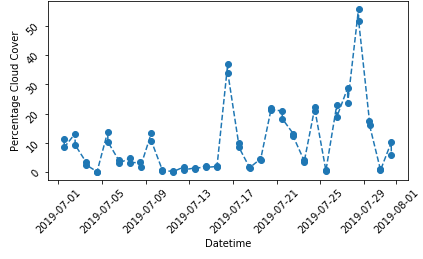
\includegraphics[totalheight=0.3\textheight]{cloud_percent_jul_southsea_not.png}
    \caption{Plot of the change in cloud cover percentage over the course of July 2019 for an area over the Atlantic Ocean in the Southern Hemisphere}
    \label{fig:cloud_pc_jul}
\end{figure}

\begin{figure}[hbt!]
    \centering
    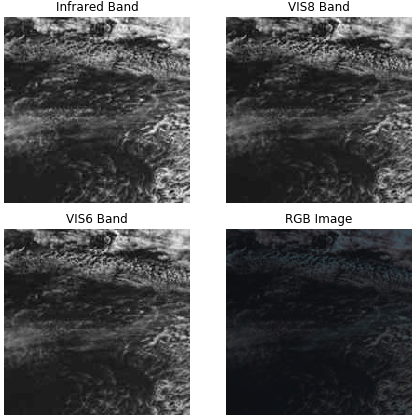
\includegraphics[width=0.6\textwidth]{0_per_day_sea_not.png}
    \caption{Images of the three channels (IR 1.6, VIS 0.8, VIS 0.6) and the calculated RGB image for 2019-07-04 12:27:43}
    \label{fig:0pc}
\end{figure}

Fig.~\ref{fig:cloud_pc_jul}, like Fig.~\ref{fig:cloud_pc_jan}, shows a plot of percentage cloud cover change over the month of July 2019, with percentage values ranging from approximately 0 to nearly 60, although the percentage cloud cover for the majority of the days can be seen to be between 0 and 20 percent. 

\subsection{NDVI}

\begin{figure}[H]
    \centering
    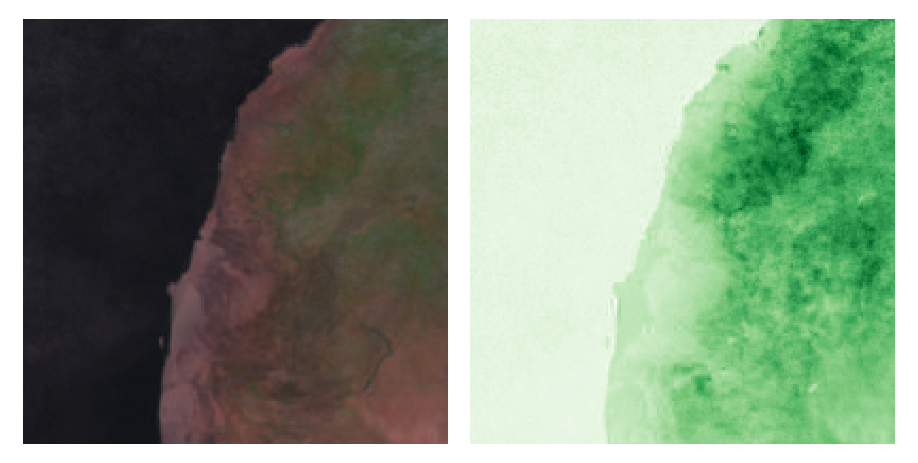
\includegraphics[width=0.7\textwidth]{ndvi_av_jan+av_jan.png}
    \caption{(Left) Plot of NDVI calculated values per pixel from the cloud free averaged image in January. (Right) Plot showing density of green vegetation. Darker green areas show higher concentration of vegetation and biomass.}
    \label{fig:ndvi_jan_av}
\end{figure}

Fig.~\ref{fig:ndvi_jan_av} makes use of the monthly averaged RGB image and Equation.~\ref{eq:ndvi} to show both the cloud free averaged RGB value for the month of January 2019 and the calculated NDVI values for each pixel for this image. The darker areas towards the top right hand corner of the right hand image correspond to larger positive NDVI values indicative of vegetation, while the lightest values on the left hand side of the image indicate vegetation free surfaces.

\begin{figure}[H]
    \centering
    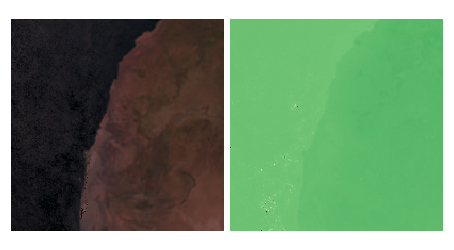
\includegraphics[width=0.7\textwidth]{ndvi_av_jul+av_jul.png}
    \caption{(Left) Plot of NDVI calculated values per pixel from the cloud free averaged image in July. (Right) Plot showing density of green vegetation skewed by outlier pixels. Darker green areas show higher concentration of vegetation and biomass.}
    \label{fig:ndvi_jul_av}
\end{figure}

Fig.~\ref{fig:ndvi_jul_av} makes use of the monthly averaged RGB image and Equation.~\ref{eq:ndvi} to show both the cloud free averaged RGB value for the month of July 2019 and the calculated NDVI values for each pixel for this image. Due to minimal cloud cover in July the cloud detection and removal method used made use of the inspection threshold values.